\problemname{Storstad}

Deltagarna i den svenska programmeringsolympiaden älskar geometri, och det med rätta. Den största favoriten bland geometrierna är den så kallade \emph{manhattangeometrin}. Manhattanavståndet mellan två punkter \textbf{P} och \textbf{Q} i ett regelbundet rutnät beskriver hur många punkter man måste passera för att ta sig från \textbf{P} till \textbf{Q}, givet att man bara får gå horisontellt och vertikalt.

Om \textbf{P} $= (x_1,y_1)$ och \textbf{Q} $= (x_2,y_2)$, så beräknas manhattanavståndet mellan punkterna som $|x_1-x_2| + |y_1-y_2|$. $|a|$ betecknar absolutbeloppet för talet $a$, dvs vi ignorerar minustecknet om talet är negativt.

Nu är det dags för dig att visa hur mycket du älskar geometri. Du ska planera din flytt till en storstad där manhattanavstånd gäller. Du har $N$ stycken vänner som bor i storstaden, men du har bara $M$ lägenheter att välja på. Din uppgift är att lista ut hur du ska välja lägenhet så att summan av manhattanavstånden till alla dina $N$ vänner från din lägenhet är \emph{så liten som möjligt}.

\section*{Delpoäng}
På det här problemet kan du samla poäng trots att du inte löser problemet helt och hållet.

\begin{itemize}
\item För 40\% av poängen gäller att $1 \leq N \leq 10^4$ och $1 \leq M \leq 100$.
\item För full poäng måste din lösning hantera $1 \leq N \leq 10^5$ och $1\leq M \leq 10^5$.
\end{itemize}

\begin{figure}[!h]
\begin{center}
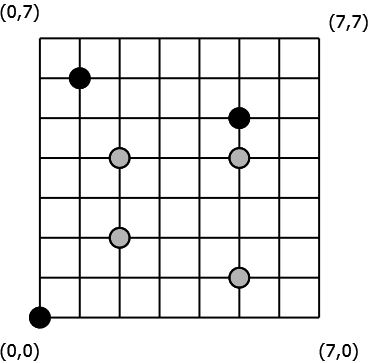
\includegraphics[scale=0.4]{Storstad}
\end{center}
\caption{De svarta prickarna representerar lägenheter vi kan välja på i storstaden, och de grå prickarna markerar var våra vänner bor. Om vi väljer lägenheten i (0,0) så blir summan av avstånden till vännerna 4+6+6+9=25. Väljer vi lägenheten i (1,6) så blir summan av avstånden 3+5+6+9=23. Väljer vi den sista lägenheten så blir summan av avstånden 1+4+6+4=15, och att välja lägenheten i (5,5) är då optimalt.}
\label{fig1}
\end{figure}

\section*{Indata}
På första raden i indata finns två heltal $N$ och $M$, separerade av ett mellanslag. Sedan följer $N$ rader med två par av heltal $-10 000 \leq x_i \leq 10 000$ och $-10 000 \leq y_i \leq 10 000$, separerade av mellanslag. Dessa beskriver på vilka korsningar i staden som dina vänner bor. Slutligen följer M rader med par av tal $-10 000 \leq x_i \leq 10 000$ och $-10 000 \leq y_i \leq 10 000$, separerade av mellanslag, som beskriver på vilka korsningar i staden du kan välja att bo. Notera att det kan finnas flervåningshus i storstaden (en punkt kan förekomma flera gånger i indata).

\section*{Utdata}
Ditt program ska skriva ut ett enda tal på en rad: den minsta möjliga summan av manhattanavstånden till dina $N$ vänner från din lägenhet.
